\documentclass[11pt,letterpaper]{article}
\usepackage[margin=1.0in]{geometry}
\usepackage[utf8]{inputenc}
\usepackage{cite}
\usepackage{amsmath}
\usepackage{amsfonts}
\usepackage{amssymb}
\usepackage{makeidx}
\usepackage{graphicx}
\usepackage{color}
\setlength\parindent{0pt}
\usepackage[framed,numbered,autolinebreaks,useliterate]{mcode}

\author{STUDENT NAME}
\title{HW: Thevenin Equivalents}

\begin{document}

\maketitle

This homework contains three worked examples of increasing complexity, and three examples that you need to do. Although the examples all have numbers, you need to submit equations. Many students do not like homeworks without numbers, but the reality is that you need to have equations before you can plug in numbers anyway, so asking for numbers is only more work. In fact, the best way to solve these kinds of problems is to first write out the equations and then write a simple MatLab script to do the calculations!\\

The procedure of the Thevenin Equivalent method is as follows:

\begin{enumerate}
\item Determine the Open Voltage across a,b (note ground symbol)
\item With all sources replaced by their internal resistance, calculate the circuit's Equivalent Resistance that a ohm meter would "see" at a,b.
\item Determine the circuit's short current through a-b by drawing in a direct connection between a,b.
\item Verify your answer using Ohm's Law: $U_{open} = R_{eq} * i_{short}$
\end{enumerate}

As you will see in the three worked examples, you need to determine the equations for the Open Voltage, Equivalent Resistance and the Short Current. To get numerical values, we need to write a simple MatLab program. This is much faster than doing it on paper, and the computer does not make any mistakes. First we need a function called 'parallel' so we can calculate the equivalent value of two resistors in parallel: Copy these two lines in MatLab's editor and save as 'parallel.m'. As you can see it simply takes two resistors and applies the 'product over sum' rule. Now you can use this function in your homework.

\begin{lstlisting}
function Rout = parallel(R1, R2)
Rout = R1*R2/(R1 + R2);
\end{lstlisting}

\newpage

\textbf{Worked example 1}

Figure \ref{fig:HW_Thevenin1} shows the circuit. It is easy to see that the two resistors make up a voltage divider. Since the Open Voltage is the voltage across resistor $R_2$, it is now the resistor itself, divided by the sum of the two resistors, and multiplied by the voltage drop across both of them (note that the voltage on the bottom end is zero (ground symbol) but this is not always the case!)\\

To determine the equivalent resistance, you replace the voltage source by its internal resistance (which is zero). Now it is easy to recognize that the equivalent resistance is the parallel circuit made up by the two resistors.\\

To calculate $i_{short}$ you imagine point a,b being connected and the current flowing from a to b is the $i_{short}$). If you connect a wire in parallel with $R_2$, $R_2$ no longer plays a role (the resistance of any resistor in parallel with a zero resistance is that zero resistance.) Now the short current $i_{short}$ is the voltage drop across $R_1$ divided by $R_1$ itself:

\begin{figure}
\centering
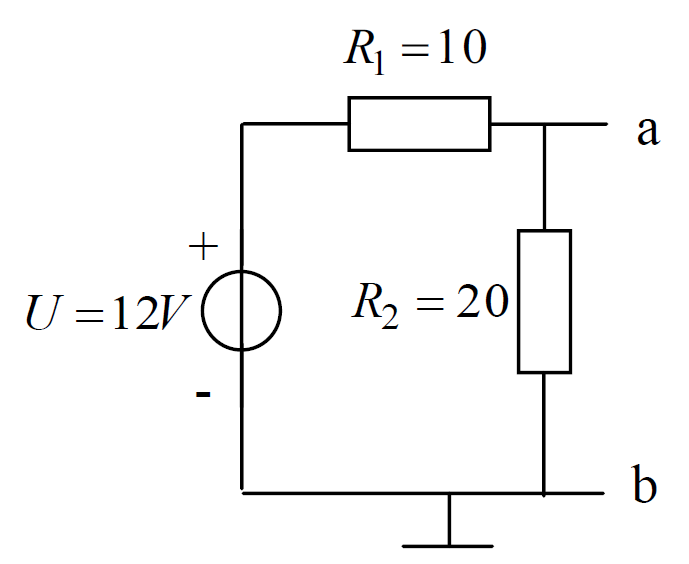
\includegraphics[width=0.4\linewidth]{HW_Thevenin1}
\caption{This circuit has a single source $U$, and two resistors $R_1$ and $R_2$. Note that this is a voltage divider circuit.}
\label{fig:HW_Thevenin1}
\end{figure}

\begin{align}\label{Eqn:HW_Thevenin1}
U_{open} &= \dfrac{R_2}{R_2+R_1} U \\
R_{eq}  &= \dfrac{R_2 R_1}{R_2 + R_1} \\
i_{short} &=  \dfrac{U}{R_1}\\
\end{align}

Check:

\begin{equation}
U_{open} = R_{eq} * i_{short} = \dfrac{R_2 R_1}{R_2 + R_1} * \dfrac{U}{R_1} = \dfrac{R_2}{R_2+R_1} U
\end{equation}

Now you write a program (which calls the 'parallel' function) as follows: Remember that every time you want to put two resistors $R_1, R_2$ in parallel simply call 'parallel(R1,R2)'.\\

\newpage
The listing of the program for worked example 1 is given here:

\begin{lstlisting}
clear all
close all
clc

U              = 12;
R1             = 10;
R2             = 20;

Uopen          = U*R2/(R1+R2)
Req            = parallel(R1, R2)
i_short        = U/R1

i_short_check  = Uopen / Req
\end{lstlisting}

The output of this program is:

\begin{lstlisting}
Uopen 			=    8
Req 			=    6.6667
i_short 		=    1.2000

i_short_check 	=    1.2000
\end{lstlisting}


\textbf{Worked example 2}

Figure \ref{fig:HW_Thevenin2} shows a circuit that contains a single current source. To calculate the Open Voltage, you have to recognize that there is no current flowing through resistor $R_2$ and therefore there is no voltage DROP across $R_2$, in other words, the voltage left and right of the resistor are the same. The voltage drop across $R_1$ is according to Ohm's law equal to $i R_1$, which is then also the voltage at point a.\\

The equivalent resistance $R_{eq}$ is easy to see, since you need to replace the current source with its internal resistance (which is infinite), therefore the $R_{eq}$ is the sum of the two resistors (since they are in series.)\\

To calculate $i_{short}$ you need to recognize that this becomes a current divider (imagine point a,b connected and the current flowing from a to b is the $i_{short}$). So the current through the $R_2$ branch is now the opposite resistor divided by the sum of the resistors, multiplied by the current entering them:

\begin{figure}
\centering
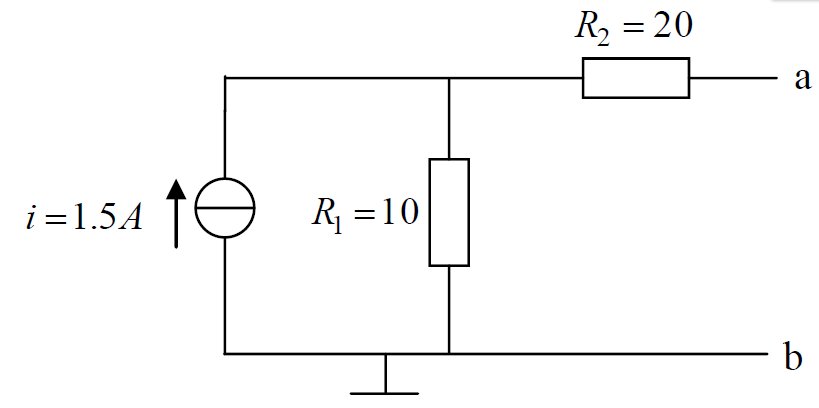
\includegraphics[width=0.65\linewidth]{HW_Thevenin2}
\caption{This circuit has a single current source $i$, and two resistors.}
\label{fig:HW_Thevenin2}
\end{figure}

\begin{align}\label{Eqn:HW_Thevenin2}
U_{open} &= i R_1 \\
R_{eq}  &= R_1 + R_2 \\
i_{short} &=  \dfrac{R_1}{R_1+R_2} i\\
\end{align}

Check:

\begin{equation}
U_{open} = R_{eq} * i_{short} = \left( R_1 + R_2\right)  \dfrac{R_1}{R_1+R_2} i = i R_1
\end{equation}

\newpage
The listing of the program for worked example 2 is given here:

\begin{lstlisting}
clear all
close all
clc

i              = 1.5;

R1             = 10;
R2             = 20;

Uopen          = i*R1
Req            = R1+ R2
i_short        = i*R1/(R1+R2)

i_short_check  = Uopen / Req
\end{lstlisting}

The output of this program is:

\begin{lstlisting}
Uopen 			=   15
Req 			=   30
i_short 		=   0.5000

i_short_check 	=   0.5000
\end{lstlisting}

\newpage

\textbf{Worked example 3}
Figure \ref{fig:HW_Thevenin3} shows the circuit. Here is where things get a litte more difficult, since we now have two sources, a voltage source and a current source. The trick is to use the super position principle to determine the Thevenin equivalent. What this boils down to is that during the calculation of $U_{open}$, you calculate the influence of the voltage source (while temporarily replacing the current source by its internal resistance, which is infinite) and then you do the opposite, you calculate the influence of the current source (while temporarily replacing the voltage source by its internal resistance, which is zero). Then you simply add the two influences. You do the exact same thing for the short current $i_{short}$. However you do not need to do this for the equivalent resistance, since it is not a source; You calculate the equivalent resistance by replacing both sources by their internal resistance.\\

For circuits like these, it is best to split it into two parts, 1) where you only have a voltage source and 2) where you only have a current source (see Figures \ref{fig:HW_Thevenin3_VoltageSource} and \ref{fig:HW_Thevenin3_CurrentSource}). Once you get good at this, you think you can see it in your head, but people are limited in the number of variables they can oversee at once. It is much better to be systematic than to rely on intuition!\\


\begin{figure}
\centering
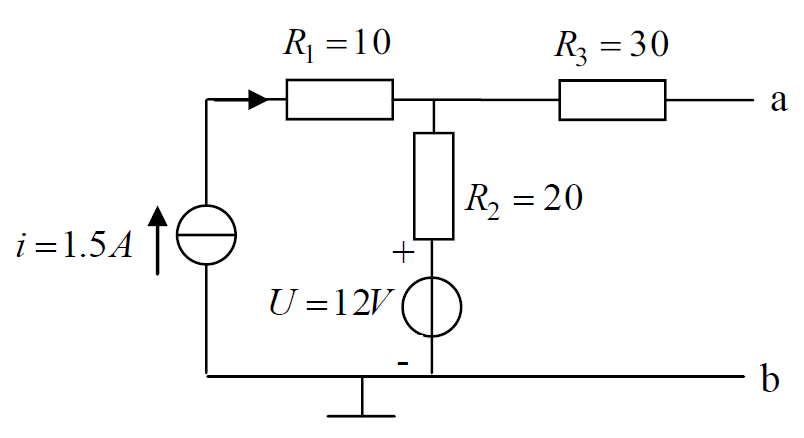
\includegraphics[width=0.65\linewidth]{HW_Thevenin3}
\caption{This circuit has one voltage source and one current source. Unless you are some math savant, you will not be able to see the equations unless you redraw this circuit into two parts, 1) taking only into account the influence of the voltage source, and 2) taking only into account the influence of the current source.}
\label{fig:HW_Thevenin3}
\end{figure}

Figure \ref{fig:HW_Thevenin3_VoltageSource} shows the circuit where the current source is replaced by its internal resistance, which is infinite, therefore the whole source simply disappears.\\
\begin{figure}
\centering
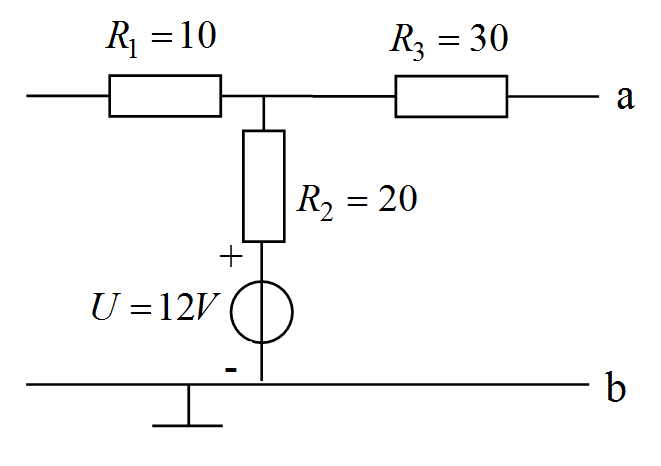
\includegraphics[width=0.5\linewidth]{HW_Thevenin3_VoltageSource}
\caption{Same circuit as shown in Figure \ref{fig:HW_Thevenin3} with only the voltage source.}
\label{fig:HW_Thevenin3_VoltageSource}
\end{figure}

By now you should be able to determine the $U_{open}, R_{eq}, and i_{short}$ of the circuit. Since there is no current flowing in the entire circuit, it is clear that the voltage at point a, is equal to the voltage above the voltage source which is $U$.\\

The equivalent resistance is also simple, because any meter hooked up to point a,b will see two resistors in series ($R_1$ plays no role since there is no current running through it).\\

The short current is now the current flow through $R_2$ and $R_3$ which is equal to the voltage source divided by the sum of resistors  $R_2$ and $R_3$:

\begin{align}\label{Eqn:HW_Thevenin3}
U_{open} &= U \\
R_{eq}  &= R_2 + R_3 \\
i_{short} &=  \dfrac{U}{R_2+R_3}\\
\end{align}

Check:

\begin{equation}
U_{open} = R_{eq} * i_{short} = \left( R_2 + R_3 \right) \dfrac{U}{R_2+R_3} = U
\end{equation}


Figure \ref{fig:HW_Thevenin3_CurrentSource} shows the circuit where the voltage source is replaced by its internal resistance, which is zero, therefore the source is replaced by a wire.\\

\begin{figure}
\centering
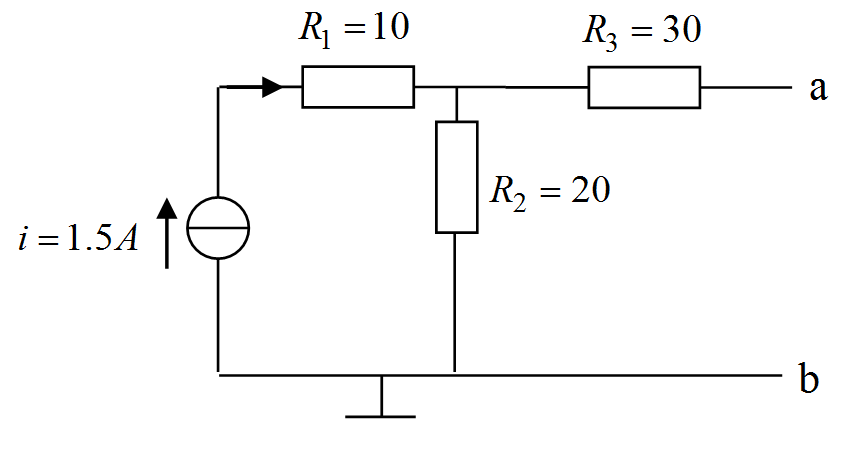
\includegraphics[width=0.65\linewidth]{HW_Thevenin3_CurrentSource}
\caption{Same circuit as shown in Figure \ref{fig:HW_Thevenin3} with only the current source.}
\label{fig:HW_Thevenin3_CurrentSource}
\end{figure}

Now we are going to determine the $U_{open}, R_{eq}$, and $i_{short}$ of this circuit. Since there is no current flowing through $R_3$, there is no voltage drop across it, and the voltage at point a is equal to the voltage to the left of resistor $R_3$. Since all current flows through $R_2$, the voltage above $R_2$ is equal to $i R_2$.\\

The equivalent resistance is equal to the one we found before, it is not a function of the sources therefore it is equal to the sum of resistors $R_2$, $R_3$.\\
 
The short current can be calculated by recognizing the current divider, and therefore the current flowing through resistor $R_3$ (which is $i_{short}$) is now equal to the opposite resistor $R_2$ divided by the sum of the resistors that make up the current divider $R_2 + R_3$  times the current running into them which is $i$.

\begin{align}\label{Eqn:HW_Thevenin4}
U_{open} &= i R_2 \\
R_{eq}  &= R_2 + R_3 \\
i_{short} &=  \dfrac{R_2}{R_2+R_3} i\\
\end{align}

Check:

\begin{equation}
U_{open} = R_{eq} * i_{short} = \left( R_2 + R_3 \right) \dfrac{R_2}{R_2+R_3} i = i R_2
\end{equation}

Since we have split the original circuit (see Figure \ref{fig:HW_Thevenin3}) into two parts, we need to add the influences of the voltage and current source separately as follows (note that the equivalent resistance $R_{eq}$ remains unaffected):

\begin{align}\label{Eqn:HW_Thevenin5}
U_{open} &= U + i R_2 \\
R_{eq}   &= R_2 + R_3 \\
i_{short} &= \dfrac{U}{R_2+R_3} +  \dfrac{R_2}{R_2+R_3} i\\
\end{align}

Check:

\begin{equation}
U_{open} = R_{eq} * i_{short} = \left( R_2 + R_3 \right) \left(  \dfrac{U}{R_2+R_3} +  \dfrac{R_2}{R_2+R_3} i\right)  = U + i R_2 
\end{equation}

\newpage
The listing of the program for worked example 3 is given here:

\begin{lstlisting}
clear all
close all
clc

U              = 12;
i              = 1.5;

R1             = 10;
R2             = 20;
R3             = 30;

Uopen          = U + i*R2
Req            = R2 + R3

i_short        = U/(R2+R3) + i*R2/(R2+R3)

i_short_check  = Uopen / Req
\end{lstlisting}

The output of this program is:

\begin{lstlisting}
Uopen 			=    42
Req 			=    50
i_short 		=    0.8400

i_short_check 	=    0.8400
\end{lstlisting}

\newpage
\textbf{Your homework starts here.}\\

Figures \ref{fig:HW_Thevenin4},  \ref{fig:HW_Thevenin5}, and \ref{fig:HW_Thevenin6} show three circuits, all of them having dual sources. Use the superposition principle to calculate the Thevenin equivalents. You do not have to insert the split circuits, but you are urged to do this on a piece of paper, and don't forget to add the influence of the separate sources at the end.\\

\textbf{To submit this homework, you need to continue this document, and solve the problems 4,5,6 in exactly the same way as was done in the worked examples. Include the equations, as well as the MatLab code.
}\\

%========================================== Circuit 4 ==========================================
\newpage
\textbf{Circuit 4 (Figure 6)}

\begin{figure}
\centering
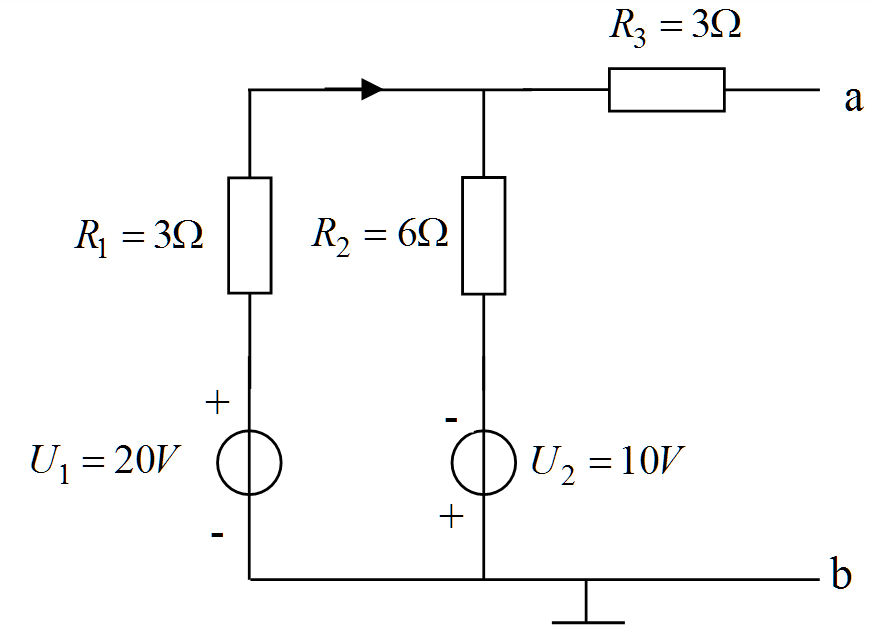
\includegraphics[width=0.65\linewidth]{HW_Thevenin4}
\caption{This circuit has two sources, $U_1$ and $U_2$. If you do not like the positive sign of source $U_2$ at the bottom, simply put it at the top, and write yourself a note that its value is $U_2' = -U_2$.}
\label{fig:HW_Thevenin4}
\end{figure}


\begin{align}\label{Eqn:HW_Thevenin6}
U_{open} &=  \\
R_{eq}  &=  \\
i_{short} &=
\end{align}

Check:

\begin{equation}
U_{open} = R_{eq} * i_{short} =
\end{equation}

\newpage
The listing of the program for circuit 4 is given here:

\begin{lstlisting}
\end{lstlisting}


The output of this program is:

\begin{lstlisting}
\end{lstlisting}

%========================================== Circuit 5 ==========================================
\newpage
\textbf{Circuit 5 (Figure 7)}

\begin{figure}
\centering
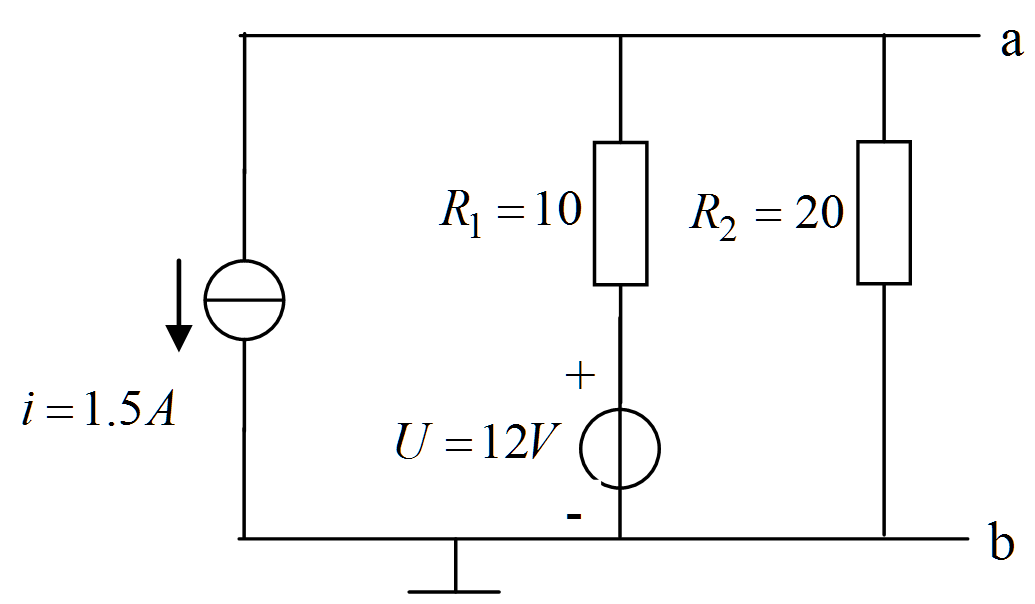
\includegraphics[width=0.65\linewidth]{HW_Thevenin5}
\caption{This circuit has a voltage and a current source, so you need to evaluate the influence of the two sources separately. Also, if you do not like the current flowing downward, simply reverse its direction and write yourself a note that says $i' = -i$.}
\label{fig:HW_Thevenin5}
\end{figure}

\begin{align}\label{Eqn:HW_Thevenin7}
U_{open} &=  \\
R_{eq}  &=  \\
i_{short} &=
\end{align}

Check:

\begin{equation}
U_{open} = R_{eq} * i_{short} =  
\end{equation}

\newpage
The listing of the program for circuit 5 is given here:

\begin{lstlisting}
\end{lstlisting}

The output of this program is:

\begin{lstlisting}
\end{lstlisting}

%========================================== Circuit 6 ==========================================
\newpage
\textbf{Circuit 6 (Figure 8)}
\begin{figure}
\centering
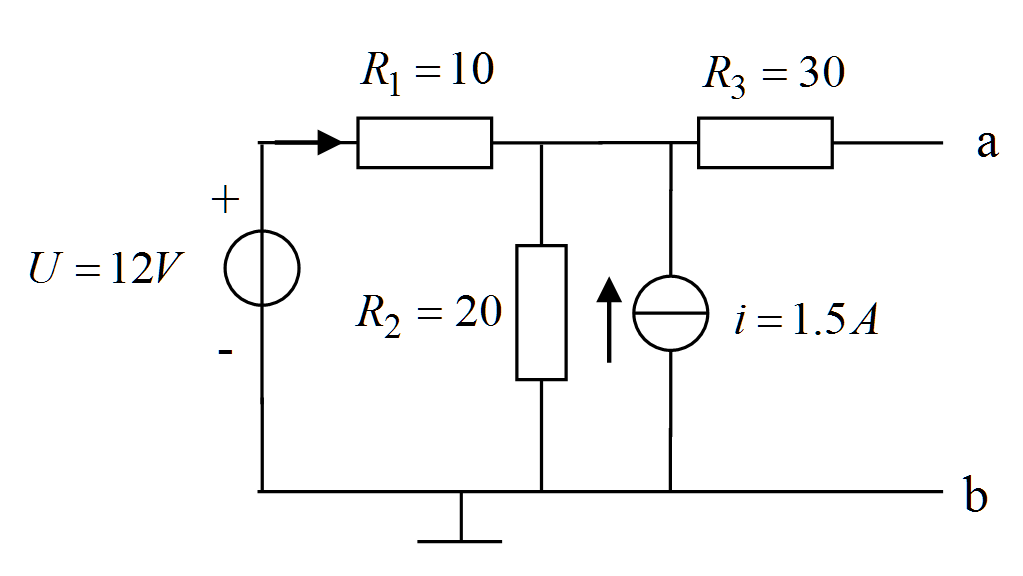
\includegraphics[width=0.65\linewidth]{HW_Thevenin6}
\caption{This circuit has two sources, use the superposition principle.}
\label{fig:HW_Thevenin6}
\end{figure}

\begin{align}\label{Eqn:HW_Thevenin8}
U_{open} &=  \\
R_{eq}  &=  \\
i_{short} &=
\end{align}

Check:

\begin{equation}
U_{open} = R_{eq} * i_{short} =
\end{equation}

\newpage
The listing of the program for circuit 6 is given here:

\begin{lstlisting}
\end{lstlisting}

The output of this program is:

\begin{lstlisting}
\end{lstlisting}


\end{document}